\documentclass[12pt,a4paper,onecolumn]{article}
\usepackage[utf8]{inputenc}
\usepackage{amsmath}
\usepackage{amsfonts}
\usepackage{amssymb}
\usepackage{graphicx}
\usepackage{ctex}
\usepackage[colorlinks=true, allcolors=blue]{hyperref}
\usepackage[left=3.00cm, right=3.00cm, top=2.00cm, bottom=2.00cm]{geometry}
\usepackage{listings}
\lstset{language=C++}%这条命令可以让LaTeX排版时将C++键字突出显示

\lstset{breaklines}%这条命令可以让LaTeX自动将长的代码行换行排版

\lstset{extendedchars=false}%这一条命令可以解决代码跨页时,章节标题,页眉等汉字不显示的问题
%\begin{lstlisting}
%\end{lstlisting}
\author{罗傲}
\title{算法笔记}
\begin{document}
	\maketitle
	\section{时间复杂度}
	时间复杂度的解释:\hyperref{https://www.iamshuaidi.com/591.html}{category}{name}{https://www.iamshuaidi.com/591.html}
	\section{排序}
	\hyperref{https://blog.csdn.net/struggle_kid/article/details/107933623}{category}{name}{C/C++中四种排序算法的时间空间复杂度}
	\subsection{选择排序,时间复杂度 $O(n^2)$}
	一种最简单的排序算法是这样的:首先,找到数组中最小的那个元素,其次,将它和数组的第
	一个元素交换位置(如果第一个元素就是最小元素那么它就和自己交换)。再次,在剩下的元素中
	找到最小的元素,将它与数组的第二个元素交换位置。如此往复,直到将整个数组排序。这种方法
	叫做选择排序,因为它在不断地选择剩余元素之中的最小者。
	\hyperref{https://github.com/la1993628/Algorithm_study/blob/master/%E9%80%89%E6%8B%A9%E6%8E%92%E5%BA%8F/a.cpp}{category}{name}{选择排序C++实现点这}
	\subsection{插入排序,时间复杂度 $O(n^2)$}
	通常人们整理桥牌的方法是一张一张的来,将每一张牌插入到其他已经有序的牌中的适当位置。
	在计算机的实现中,为了给要插入的元素腾出空间,我们需要将其余所有元素在插入之前都向右移
	动一位。这种算法叫做插入排序。
	
	与选择排序一样,当前索引左边的所有元素都是有序的,但它们的最终位置还不确定,为了给
	更小的元素腾出空间,它们可能会被移动。但是当索引到达数组的右端时,数组排序就完成了。
	
	和选择排序不同的是,插入排序所需的时间取决于输入中元素的初始顺序。例如,对一个很大
	且其中的元素已经有序(或接近有序)的数组进行排序将会比对随机顺序的数组或是逆序数组进行
	排序要快得多。
	\begin{figure}[ht]
		\centering
		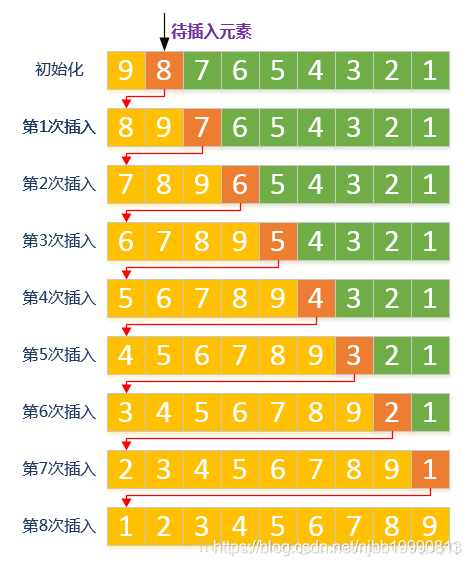
\includegraphics[width=0.7\linewidth]{img/insertSort}
		\caption{插入排序}
		\label{fig:insertsort}
	\end{figure}
\hyperref{https://github.com/la1993628/Algorithm_study/blob/master/%E6%8F%92%E5%85%A5%E6%8E%92%E5%BA%8F/a.cpp}{category}{name}{插入排序C++实现点这}
	
	
\end{document}
















